\documentclass[a4paper]{article}
\usepackage[utf8]{inputenc}
%\usepackage[T1]{fontenc}
\usepackage[french]{babel}
\frenchbsetup{FrenchFootnotes=false}
\usepackage[hang,flushmargin]{footmisc}

\usepackage{wrapfig}

% FONTS
\renewcommand{\familydefault}{\sfdefault}
\usepackage{biolinum}
\usepackage{euler}
\usepackage{inconsolata}

\usepackage{xcolor}
\usepackage{sectsty}

\usepackage{tocloft}
%\usepackage[nottoc,notlof,notlot]{tocbibind}

\definecolor{brick}{rgb}{0.6,0,0}

\sectionfont{\color{brick}}
\subsectionfont{\color{brick}}
\subsubsectionfont{\color{brick}}
\renewcommand{\footnotelayout}{\color{brick}}
\renewcommand\thefootnote{\textcolor{brick}{\arabic{footnote}}}

\usepackage{amsmath}
\usepackage{bm}
\usepackage{cancel}
\usepackage{tabu}
\usepackage{mathtools}
\usepackage{fixltx2e}
\usepackage
    [ colorlinks=true,
      linkcolor=brick,
      citecolor=brick,
      urlcolor=brick,
      linktoc=all
    ] {hyperref}

\usepackage[backend=bibtex]{biblatex}
\addbibresource{mastermind.bib}
\DeclareFieldFormat{labelnumberwidth}{\textbf{\color{brick} \{#1\}}}

\newcommand{\citewrapper}[1]{\textsuperscript{\textbf{\color{brick} \{#1\}}}}
\DeclareCiteCommand{\cite}[\citewrapper]
  {\usebibmacro{prenote}}
  {\usebibmacro{citeindex}\usebibmacro{cite}}
  {\multicitedelim}
  {\usebibmacro{postnote}}

\usepackage{tikz}
\usepackage{tikz-qtree}
\usetikzlibrary{babel}

\newcommand{\netree}{
  \begin{tikzpicture}
    [ baseline=(current bounding box.center),
      execute at begin node=\(,
      execute at end node=\),
      edge from parent/.style={draw=none} ]
    \Tree
}
\newcommand{\tree}{
  \begin{tikzpicture}
    [ baseline=(current bounding box.center),
      execute at begin node=\(,
      execute at end node=\) ]
    \Tree
}
\newcommand{\donetree}{
  \end{tikzpicture}
}

\usepackage{parskip}
\usepackage{enumitem}

\setlist[itemize]{leftmargin=*,topsep=0pt,partopsep=0pt,parsep=3pt,itemsep=0pt}

\renewcommand{\theequation}{\textbf{\arabic{equation}}}
\newtagform{brackets}{\textbf{[}}{\textbf{]}}
\usetagform{brackets}

\newcommand{\isep}{\,..\,}

\usepackage{amssymb}
\renewcommand{\emptyset}{\varnothing}

\renewcommand{\(}{\begin{math}\color{brick}}
\renewcommand{\)}{\end{math}}

\relpenalty=10000
\binoppenalty=10000

\newcommand{\blockmath}[1]{{\color{brick}\begin{align*}#1\end{align*}}}
\newcommand{\nblockmath}[1]{{\color{brick}\begin{align}#1\end{align}}}

\renewcommand{\eqref}[1]{\color{brick}\textbf{[\ref{#1}]}}
\newcommand{\seqref}[1]{\textsuperscript{\eqref{#1}}}

\renewcommand\footnoterule{\vspace{17pt} {\color{brick} \hrule height 0.5pt} \vspace{2pt}}

\newcommand{\lnd}{\,\land\,}

\newcommand{\TODO}{\colorbox{black}{\textbf{\texttt{\large\color{white}TODO}}}}

\newcommand{\srcref}[1]{\href{https://github.com/timjrd/mastermind/blob/master/#1}{\texttt{#1}}}

% TOC
\renewcommand{\cftsecleader}{\hspace{2em}}
\renewcommand{\cftsecafterpnum}{\cftparfillskip}
\renewcommand{\cftsecpagefont}{\normalfont\itshape}

\renewcommand{\cftsubsecleader}{\hspace{2em}}
\renewcommand{\cftsubsecafterpnum}{\cftparfillskip}
\renewcommand{\cftsubsecpagefont}{\normalfont\itshape}

\renewcommand{\cftsubsubsecleader}{\hspace{2em}}
\renewcommand{\cftsubsubsecafterpnum}{\cftparfillskip}
\renewcommand{\cftsubsubsecpagefont}{\normalfont\itshape}

\newcommand{\ttl}[1]{{\Large\color{brick}#1}}
\newcommand{\vsp}{\vspace{0.3cm}}

\renewcommand{\cftpnumalign}{l}

\title{Programme-joueur de \\ Mastermind paramétrique}
\author{Timothée Jourde}

\begin{document}

\setlength{\abovedisplayskip}{0pt}
\setlength{\belowdisplayskip}{0pt}
\setlength{\abovedisplayshortskip}{0pt}
\setlength{\belowdisplayshortskip}{0pt}

%\usetagform{arabic}

%\maketitle

\begin{titlepage}
  \centering
  \large

  {
    Université de Bordeaux
  }
  
  \vfill

  {
    \ttl{\Huge Programme-joueur de \\ Mastermind paramétrique}

    \vsp
    
    \ttl{Stage de première année de Master Informatique}
  }
  
  \vfill

  {
    \textit{Timothée Jourde}
  }
         
  \vfill

  {
    \ttl{Maîtres de stage}
    
    \vsp
    
    \textit{Hugo Gimbert \\ Nathanaël Fijalkow}
    
    \vsp
    
    Laboratoire Bordelais de \\ Recherche en Informatique
  }
  
  \vfill

  {
    \ttl{Enseignant référent}
    
    \vsp
    
    \textit{Grégoire Passault}
  }
  
  \vfill

  {
    \today
  }
\end{titlepage}

\clearpage

{\color{brick}\tableofcontents}

\section{Introduction}

\begin{wrapfigure}{r}{11em}
  \vspace{-\baselineskip}
  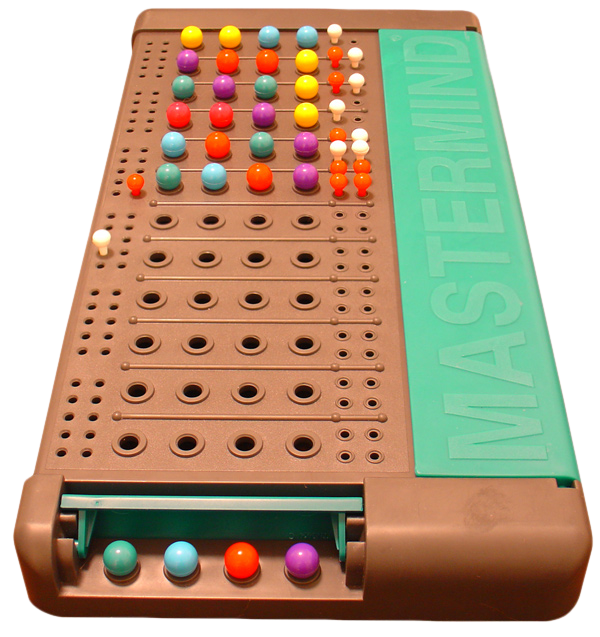
\includegraphics[width=11em]{mastermind.png}
\end{wrapfigure}

Le Mastermind\footnote{\url{https://en.wikipedia.org/wiki/Mastermind_(board_game)}} est un jeu de logique où l'un des deux joueurs doit deviner un code secret à partir des indications données par l'autre joueur. La version originale du Mastermind se joue avec un code de quatre pions colorés choisis parmi un ensemble de six couleurs.

L'objectif de ce stage est de réaliser un programme-joueur de Mastermind, avec une taille de code et un nombre de couleurs paramétrables à l'exécution.

\section{Objectif}

\subsection{Formalisation du jeu}

On formalise une partie de Mastermind par :

\begin{itemize}
  
\item une taille de combinaison \(n\)
  
\item un nombre de couleurs \(m\)
  
\item une combinaison secrète \(c_s : [1 \isep n] \rightarrow [1 \isep m]\)
  
\item une suite de tentatives \((c_i, h(c_s,c_i))\), où :
  
  \begin{itemize}
    
  \item \(i \in [1 \isep ]\) est la tentative
    
  \item \(c_i : [1 \isep n] \rightarrow [1 \isep m]\) est la combinaison jouée
    
  \item \(h(s,c) = (g,b)\) est la fonction associant une indication \((g,b)\) à une combinaison secrète \(s\) et à une combinaison jouée \(c\), où :
    
    \begin{itemize}
      
    \item \(g\) est le nombre de couleurs de \(c\) correspondant
      à celles de \(s\) et à la même position (couleurs ``bien
      placés'').
      
      \blockmath{
        g = \sum_{j=0}^{n}
        \begin{cases}
          1 & \text{si } c(j)=s(j) \\
          0 & \text{sinon}
        \end{cases}
      }
      
    \item \(b\) est le nombre de couleurs de \(c\) correspondant
      à celles de \(s\) mais pas à la même position (couleurs ``mal
      placés'').
      
      \blockmath{
        b = \sum_{j=0}^{n}
        \begin{cases}
          1 & \text{si } c(j) \in s[[1 \isep n]] \lnd c(j) \neq s(j) \\
          0 & \text{sinon}
        \end{cases}
      }
      
    \end{itemize}
  \end{itemize}
\end{itemize}

L'un des deux joueurs décide de \(c_s\) et donne les indications à
chaque tentative de l'autre joueur. Le joueur donnant les indications est
donc passif et peut être remplacé par un programme trivial. Le but du
jeu étant, pour l'autre joueur, de deviner \(c_s\) en un minimum de
tentatives.

\subsection{Présentation de l'algorithme}

On souhaite réaliser un programme-joueur de Mastermind (avec \(n\) et \(m\) paramétrables) capable de deviner \(c_s\) en un nombre raisonable de tentatives. L'algorithme présenté ci-après est inspiré d'une méthode\cite{sat} mise au point par Miroslav Klimoš et Antonín Kučera.

Pour un \(n\) et \(m\) fixé, on pose :

\begin{itemize}
  
\item \(C\) l'ensemble des combinaisons.
  
\item \(C_i\) l'ensemble des combinaisons privé des combinaisons déjà jouées lors des tentatives précédentes à la tentative \(i\) (combinaisons candidates).
  
  \blockmath{
    C_i = C \setminus \{c_j \mid j \in [1 \isep i-1]\}
  }

\item \(S_i\) l'ensemble des combinaisons secrètes possibles à la tentative \(i\).
  
  \nblockmath{ \label{pred}
    S_i = \{s \mid s \in C \lnd j \in [1 \isep i-1] \lnd h(s,c_j) = h(c_s,c_j)\}
  }

\item \(K_i\) : pour chaque combinaison \(c\) de \(C\), on génère un ensemble d'indications \((s,h(s,c))\) avec chaque combinaison secrète \(s\) de \(S_i\).
  
  \nblockmath{ \label{prod}
    K_i = \{ \ (c, \ \{(s,h(s,c)) \mid s \in S_i\}) \ \mid \ c \in C_i \ \}
  }

\end{itemize}

On associe un score \(k(K_c)\) à chaque combinaison, et on déduit la prochaine combinaison jouée \(c_i\) du score maximal.

\blockmath{
  c_i = c \mid (c,K_c) \in K_i \lnd (c',K_c') \in K_i \lnd k(K_c) \geq k(K_c')
}

Le choix de la fonction \(k\) associant un score à un ensemble d'indications \(K_c\) déterminera la façon dont l'algorithme convergera. On peut simplement choisir le cardinal de l'ensemble sans tenir compte des combinaisons secrètes \(s\) associés. Cela aura pour effet de maximiser le fractionnement de \(S_i\) dans le cas moyen.

\blockmath{
  k(K_c) = | \ \{ h' \mid (s,h') \in K_c\} \ |
}


\section{Réalisation}
\label{random}

Nous allons maintenant nous focaliser sur les étapes clefs de l'algorithme décrit précédement et en expliquer l'implémentation. Les sources de ce programme écrit en Haskell\footnote{\url{https://www.haskell.org}} sont disponibles en ligne : \url{https://github.com/timjrd/mastermind}.

Tel que nous l'avons décrit, l'algorithme nécessite de calculer un produit cartésien\seqref{prod} \(K_i\) entre \(C_i\) et \(S_i\), or cette opération est très coûteuse et nécessite d'énumérer complétement les deux ensembles, ce qui devient hors de portée lorsque \(n\) et \(m\) sont trop grands. On approxime donc \(K_i\) par une méthode de type monte-carlo en énumérant seulement un sous-ensemble randomisé de \(C_i\) et de \(S_i\).

\subsection{Énumération des combinaisons candidates}

Voir \srcref{src/Mastermind/Candidate.hs}.

On cherche à énumérer un sous-ensemble randomisé de \(C_i\). On génère pour cela une suite de combinaisons aléatoires, et on vérifie simplement que chaque nouvelle combinaison est unique et n'a pas déjà été jouée.

\subsection{Énumération efficace des combinaisons secrètes}

On cherche à énumérer un sous-ensemble randomisé de \(S_i\). On peut aborder le problème de la même manière que pour \(C_i\) : générer une suite de combinaisons aléatoires \(s\) et vérifier que chacune satisfasse \(h(s,c_j) = h(c_s,c_j)\)\seqref{pred}. Cette première approche a été implémentée mais s'est révélée impraticable au delà d'un certain \(n\) et \(m\).

Il a donc fallu chercher une autre solution : déduire directement \(S_i\) des tentatives précédentes (contraintes). La méthode ainsi retenue se déroule en deux étapes : l'énumération des ``permutations d'indications'', puis la génération des combinaisons secrètes à partir de ces permutations. Nous illustrerons cette section par l'exemple suivant :

\blockmath{
  n = 3 \quad m = 3 \quad
  \begin{tabu}{|c|c|c|}
    \everyrow{\hline}\hline
    c_s(1) & c_s(2) & c_s(3) \\
    3      & 1      & 3      \\
  \end{tabu} \quad 
  \begin{tabu}{|c|c|c|c|c|}
    \everyrow{\hline}\hline
    i & c_i(1) & c_i(2) & c_i(3) & h(c_s,c_i) \\
    1 & 2      & 3      & 1      & (0,2)      \\
    2 & 3      & 2      & 2      & (1,0)      \\
  \end{tabu}
}

\subsubsection{Permutations d'indications}
\label{perm}

Voir \srcref{src/Mastermind/Permutation.hs}.

La première étape consiste à représenter les indications sous la forme de séquences d'étiquettes. \(G\) pour une bonne couleur bien placée, \(B\) pour une bonne couleur mal placée, \(W\) pour une mauvaise couleur. Appliquons ceci à notre exemple :

\blockmath{
  h(c_s,c_1) &= (0,2) \equiv P(BBW) \\
  h(c_s,c_2) &= (1,0) \equiv P(GWW)
}

Ici \(n = 3\) : on obtient donc une séquence de trois étiquettes par combinaison jouée. En associant une séquence à sa combinaison, on associe dans l'ordre une étiquette à chaque membre\footnote{couleur et position} de la combinaison, et on exprime ainsi le fait qu'un membre en particulier est bien placé, mal placé, ou absent de la combinaison secrète. Une indication n'est cependant pas équivalente à une séquence particulière \(x\), mais à l'ensemble de ses permutations \(P(x)\), que l'on construit grâce à un arbre de permutation \(T(x)\) :

\blockmath{
  T(BBW) = \tree [
    [.B
      [.B
        [.W
        ]
      ]
      [.W
        [.B
        ]
      ]
    ]
    [.W
      [.B
        [.B
        ]
      ]
    ]
  ] \donetree \qquad  
  T(GWW) = \tree [ [.G [.W W ] ] [.W [.G W ] [.W G ] ] ] \donetree
}

On cherche maintenant à élaguer ces arbres pour ne conserver que les permutations valides au regard de l'ensemble des contraintes (une contrainte correspondant à un arbre). Il faut donc mettre en relation ces différents arbres, on procède ainsi à leur concaténation :

\blockmath{
  T(BBW) \cdot T(GWW) = \tree [
    [.B
      [.B
        [.W
          [.G [.W W ] ] [.W [.G W ] [.W G ] ]
        ]
      ]
      [.W
        [.B
          [.G [.W W ] ] [.W [.G W ] [.W G ] ]
        ]
      ]
    ]
    [.W
      [.B
        [.B
          [.G [.W W ] ] [.W [.G W ] [.W G ] ]
        ]
      ]
    ]
  ] \donetree
}

Chaque niveau de l'arbre correspond à une position et à une couleur. Le second niveau correspond ainsi à \(c_1(2)=3\) tandis que le dernier niveau correspond à \(c_2(3)=2\). Pour élaguer l'arbre on effectue un parcours en largeur depuis la raçine en supprimant les nœuds incompatibles avec leurs ancêtres. Illustrons cette opération avec notre exemple (les couleurs correspondantes sont représentées à droite de l'arbre) :

\begin{equation*}
  \color{brick}  
  \tree [
      [.{\textsuperscript{+}B}
        [.B
          [.W
            [.G [.{\textsuperscript{+}\cancel{W}} ] ] [.\cancel{W} ]
          ]
        ]
        [.{\textsuperscript{$*$}W}
          [.B
            [.{\textsuperscript{$*$}\cancel{G}} ] [.W [.G \cancel{W} ] [.\cancel{W} ] ]
          ]
        ]
      ] \edge[ultra thick];
      [.\bm{W} \edge[ultra thick];
        [.\bm{B} \edge[ultra thick];
          [.\bm{B} \edge[ultra thick];
            [.\bm{G} \edge[ultra thick]; [.\bm{W} \edge[ultra thick]; \bm{W} ] ] [.\cancel{W} ]
          ]
        ]
      ]
  ] \donetree \qquad
  \netree [ [.2 [.3 [.1 [.3 [.2 [.2 ] ] ] ] ] ] ] \donetree
\end{equation*}

On a entre autre supprimé le nœud \(\textsuperscript{+}\cancel{W}\) puisqu'il signifie ``\(2\) est une mauvaise couleur'' alors que le nœud ascendant \(\textsuperscript{+}B\) signie de manière contradictoire ``\(2\) est une bonne couleur mal placée''. De même, on a supprimé \(\textsuperscript{$*$}\cancel{G}\) qui signifie ``\(3\) est une bonne couleur bien placée'' alors que \(\textsuperscript{$*$}W\) signifie ``\(3\) est une mauvaise couleur''. Le chemin en gras est entièrement valide, on retiendra donc cette séquence d'étiquettes pour l'étape suivante.

\subsubsection{Génération des combinaisons secrètes}

Voir \srcref{src/Mastermind/Secret.hs}.

On retient donc la séquence d'étiquettes \(WBBGWW\), soit \(WBB\) pour \(c_1\) et \(GWW\) pour \(c_2\). Pour chaque position de chaque combinaison, on détermine l'éventuelle couleur requise ainsi que les éventuelles couleurs exclues. On détermine également les couleurs requises sur l'ensemble d'une combinaison. On agrège ensuite les différentes contraintes ainsi obtenues.

\blockmath{
  \begin{tabu}{|r|c|c|c|}
    \everyrow{\hline}\hline
    c_1              & 2         & 3         & 1         \\
    \text{étiquette} & W         & B         & B         \\
    \text{requise}   & \emptyset & \emptyset & \emptyset \\
    \text{exclues}   & \{2\}     & \{3,2\}   & \{1,2\}   \\
    \text{requises}  & \multicolumn{3}{c|}{\{3,1\}}     \\
  \end{tabu}
  \cup
  \begin{tabu}{|r|c|c|c|}
    \everyrow{\hline}\hline
    c_2              & 3         & 2         & 2         \\
    \text{étiquette} & G         & W         & W         \\
    \text{requise}   & \{3\}     & \emptyset & \emptyset \\
    \text{exclues}   & \{2\}     & \{2\}     & \{2\}   \\
    \text{requises}  & \multicolumn{3}{c|}{\{3\}}     \\
  \end{tabu}
  =
  \begin{tabu}{|r|c|c|c|}
    \everyrow{\hline}\hline
    \text{requise}   & \{3\}     & \emptyset & \emptyset \\
    \text{exclues}   & \{2\}     & \{3,2\}   & \{1,2\}   \\
    \text{requises}  & \multicolumn{3}{c|}{\{3,1\}}      \\
  \end{tabu}  
}

Enfin, on génère le sous-ensemble \(X\) de \(S_i\) correspondant à notre séquence d'étiquettes grâce à une structure arboressante à partir des contraintes agrégées obtenues précédemment.

\begin{equation*}
  \color{brick}
  \tree [.{X \subset S_i} \edge[draw=none]; [.\bm{3}
    \edge[ultra thick]; [.\bm{1}
      \edge[dashed]; \cancel{1}
      \edge[dashed]; \cancel{2}
      \edge[ultra thick]; \bm{3}
    ]
    \edge[dashed]; \cancel{2}
    \edge[dashed]; \cancel{3}
  ] ]
  \donetree \qquad
  \netree [.\text{requise}  [.\{3\} [.{\emptyset} [.{\emptyset} ] ] ] ] \donetree \qquad
  \netree [.\text{exclues}  [.\{2\} [.\{3,2\} [.\{1,2\} ] ] ] ] \donetree \qquad
  \netree [.\text{requises} [.\{\cancel{3},1\} [.\{\cancel{1}\} [.{\emptyset} ] ] ] ] \donetree \qquad
\end{equation*}

On repète l'opération pour chaque séquence d'étiquettes obtenues à l'étape précédente.

\section{Limitations et améliorations possibles}

\subsection{Randomisation}
Comme évoqué au début de la section \ref{random}, on énumère un sous-ensemble {\em randomisé} de \(S_i\). Cette propriété est partiellement obtenue en randomisant les deux structures arborresantes utilisées. L'ordre des enfants d'un nœud est ainsi aléatoire ; on espère ainsi, lors du parcours final de l'arbre, énumérer l'ensemble correspondant dans un ordre aléatoire. Or cette technique, bien que peu coûteuse, n'offre pas une randomisation de bonne qualité, ce qui risque d'affecter les résultats de l'algorithme.

\subsection{Consommation mémoire}
Par soucis de simplification du code, on utilise deux structures de données arboressantes intermédiaires, et on exploite l'évaluation paresseuse de Haskell pour construire et consommer progressivement ces structures, à la demmande.

Au delà d'un certain \(n\) et \(m\), on observe une explosion de la consommation mémoire. Cette consommation pourrai très certainement être réduite en se passant de ces structures intermédiares, au prix d'une obfuscation du code.

\subsection{Parallélisation}
Haskell étant un langage fonctionnel pur, il n'autorise aucun changement d'état ni effet de bord. Notre programme pourrait ansi être parallélisé sans réécriture majeur. Une première approche pourrait être de calculer simultanément la génération des combinaisons secrètes à partir des différentes séquences d'étiquettes.

\section{Conslusion}

Nous avons décrit dans ce rapport la réalisation de notre programme-joueur de Mastermind paramétrique. L'objectif de ce stage a été atteint avec un programme exécutable offrant des performances bien supérieures --- et des résultats au moins équivalents --- à une approche naïve par recherche exhaustive.

Sur un plan personnel, j'ai trouvé ce stage très enrichissant puisqu'il m'a poussé à réfléchir au problème posé de manière formelle, et d'une façon approfondie. Je souhaite à ce titre remercier M. Hugo Gimbert ainsi que M. Nathanaël Fijalkow pour m'avoir donné l'opportunité de travailler sur ce sujet de stage, et pour m'avoir guider dans la réalisation du projet.

\printbibliography[heading=bibintoc]

\end{document}

